\section{Package View}
\begin{figure}[h!]
\begin{center}
	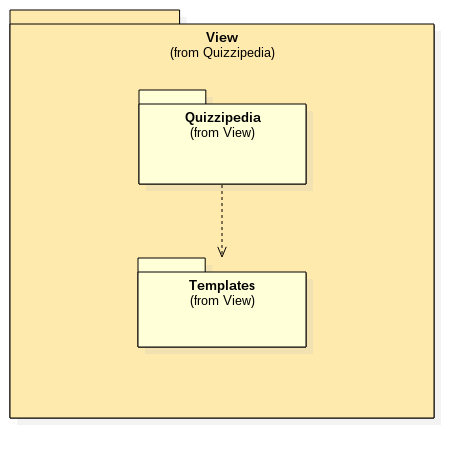
\includegraphics[scale=0.7]{../images/ViewPackage.png}
\end{center}
\end{figure}

\subsection{View::Pages}
\subsubsection{View::Pages::Page}
\begin{itemize}
\item\textbf{Funzione del componente:} rappresenta una pagina web
				\item\textbf{Relazioni d'uso con altre componenti:} L'interfaccia Page viene concretizzata dalle sue classi derivate, una rappresentativa per ogni pagina dell'applicazione\\ \\
\item\textbf{Attributi}:
	\begin{itemize}
		\item\code{- controller}: riferimento al controller della page\\
	\end{itemize}
\item\textbf{Metodi}:
	\begin{itemize}
		\item\code{+ show()}: metodo astratto che mostra il contenuto della pagina\\
	\end{itemize}
\end{itemize}

\subsubsection{View::Pages::LoginPage}
\begin{itemize}
\item\textbf{Funzione del componente:} visualizza il form di autenticazione e permette il login dell'utente. Fornisce inoltre un link alla pagina di registrazione e uno alla pagina di recupero della password 
				\item\textbf{Relazioni d'uso con altre componenti:} concretizza l'interfaccia Page da cui è diretta discendente e utilizza il template LoginForm\\ \\
La classe utilizza:
	\begin{itemize}
		\item View::Pages::Page\\
		\item View::Templates::LoginForm\\
	\end{itemize}
\item\textbf{Metodi}:
	\begin{itemize}
		\item\code{+ show()}: visualizza il form di autenticazione al sistema\\
		\textbf{Precondizioni}: viene richiesta la pagina di autenticazione. L'utente non è ancora autenticato\\
		\textbf{Postcondizioni}: viene visualizzata la pagina di autenticazione\\
	\end{itemize}
\end{itemize}

\subsubsection{View::Pages::RegistrationPage}
\begin{itemize}
\item\textbf{Funzione del componente:} visualizza il form di registrazione. Fornisce inoltre un link alla pagina di login
				\item\textbf{Relazioni d'uso con altre componenti:} concretizza l'interfaccia Page da cui è diretta discendente e utilizza il template RegistrationForm\\ \\
La classe utilizza:
	\begin{itemize}
		\item View::Pages::Page\\
		\item View::Templates::RegistrationForm\\
	\end{itemize}
\item\textbf{Metodi}:
	\begin{itemize}
		\item\code{+ show()}: visualizza il form di registrazione al sistema\\
		\textbf{Precondizioni}: viene richiesta la pagina di registrazione. L'utente non è autenticato\\
		\textbf{Postcondizioni}: viene visualizzata la pagina di registrazione\\
	\end{itemize}
\end{itemize}

\subsubsection{View::Pages::PasswordRecoveryPage}
\begin{itemize}
\item\textbf{Funzione del componente:} visualizza il form per il recupero della password
				\item\textbf{Relazioni d'uso con altre componenti:} concretizza l'interfaccia Page da cui è diretta discendente e utilizza il template PasswordRecoveryForm\\ \\
La classe utilizza:
	\begin{itemize}
		\item View::Pages::Page\\
		\item View::Templates::PasswordRecoveryForm\\
	\end{itemize}
\item\textbf{Metodi}:
	\begin{itemize}
		\item\code{+ show()}: visualizza il form per il recupero della password\\
		\textbf{Precondizioni}: viene richiesta la pagina della procedura per il recupero della password. L'utente non è autenticato\\
		\textbf{Postcondizioni}: viene visualizzata la pagina della procedura per il recupero della password\\
	\end{itemize}
\end{itemize}

\subsubsection{View::Pages::QuizCreationPage}
\begin{itemize}
\item\textbf{Funzione del componente:} visualizza il form di creazione di un nuovo questionario
				\item\textbf{Relazioni d'uso con altre componenti:} concretizza l'interfaccia Page da cui è diretta discendente e utilizza il template QuizCreationForm\\ \\
La classe utilizza:
	\begin{itemize}
		\item View::Pages::Page\\
		\item View::Templates::QuizCreationForm\\
	\end{itemize}
\item\textbf{Attributi}:
	\begin{itemize}
		\item\code{- user}: l'utente autenticato che sta creando il questionario\\
	\end{itemize}
\item\textbf{Metodi}:
	\begin{itemize}
		\item\code{+ show()}: visualizza il form per la creazione di un questionario\\
		\textbf{Precondizioni}: viene richiesta la pagina di creazione di un questionario. L'utente è autenticato\\
		\textbf{Postcondizioni}: viene visualizzata la pagina di creazione di un questionario\\
	\end{itemize}
\end{itemize}

\subsubsection{View::Pages::QuestionUpdatePage}
\begin{itemize}
\item\textbf{Funzione del componente:} visualizza il form di modifica di una domanda
				\item\textbf{Relazioni d'uso con altre componenti:} concretizza l'interfaccia Page da cui è diretta discendente e utilizza il template QuestionForm\\ \\
La classe utilizza:
	\begin{itemize}
		\item View::Pages::Page\\
		\item View::Templates::QuestionForm\\
	\end{itemize}
\item\textbf{Attributi}:
	\begin{itemize}
		\item\code{- user}: l'utente autenticato che sta modificando la domanda\\
		\item\code{- question}: la domanda da modificare\\
	\end{itemize}
\item\textbf{Metodi}:
	\begin{itemize}
		\item\code{+ show()}: visualizza il form per la modifica di una domanda compilato con i dati attuali\\
		\textbf{Precondizioni}: viene richiesta la pagina di modifica di una domanda. L'utente è autenticato\\
		\textbf{Postcondizioni}: viene visualizzata la pagina di modifica di una domanda\\
	\end{itemize}
\end{itemize}

\subsubsection{View::Pages::QuestionCreationPage}
\begin{itemize}
\item\textbf{Funzione del componente:} visualizza il form di creazione di una nuova domanda
				\item\textbf{Relazioni d'uso con altre componenti:} concretizza l'interfaccia Page da cui è diretta discendente e utilizza il template QuestionForm\\ \\
La classe utilizza:
	\begin{itemize}
		\item View::Pages::Page\\
		\item View::Templates::QuestionForm\\
	\end{itemize}
\item\textbf{Attributi}:
	\begin{itemize}
		\item\code{- user}: l'utente autenticato che sta creando la domanda\\
	\end{itemize}
\item\textbf{Metodi}:
	\begin{itemize}
		\item\code{+ show()}: visualizza il form per la creazione di una domanda\\
		\textbf{Precondizioni}: viene richiesta la pagina di creazione di una domanda. L'utente è autenticato\\
		\textbf{Postcondizioni}: viene visualizzata la pagina di creazione di una domanda\\
	\end{itemize}
\end{itemize}

\subsubsection{View::Pages::QuestionManagementPage}
\begin{itemize}
\item\textbf{Funzione del componente:} visualizza la lista delle domande create dall'utente
				\item\textbf{Relazioni d'uso con altre componenti:} concretizza l'interfaccia Page da cui è diretta discendente e utilizza il template QuestionList\\ \\
La classe utilizza:
	\begin{itemize}
		\item View::Pages::Page\\
		\item View::Templates::QuestionList\\
		\item View::Templates::Question\\
	\end{itemize}
\item\textbf{Attributi}:
	\begin{itemize}
		\item\code{- user}: l'utente autenticato che sta gestendo le proprie domande\\
		\item\code{- questions}: le domande dell'utente user\\
	\end{itemize}
\item\textbf{Metodi}:
	\begin{itemize}
		\item\code{+ show()}: visualizza la lista delle domande dell'utente permettendone la modifica e l'eliminazione. Permette inoltre di creare una nuova domanda, di ordinare la lista e fare una ricerca tra le domande\\
			\textbf{Precondizioni}: viene richiesta la pagina di gestione delle proprie domande. L'utente è autenticato\\
			\textbf{Postcondizioni}: viene visualizzata la pagina di gestione delle proprie domande\\
		\item\code{+ sort()}: ordina la lista delle domande secondo il criterio \code{by}\\
			\textbf{Precondizioni}: l'utente ha selezionato un criterio di ordinamento\\
			\textbf{Postcondizioni}: la lista di domande viene ordinata secondo il criterio inserito\\
			\textbf{Parametri}:
				\begin{itemize}
					\item\code{by}: criterio di ordinamento\\
				\end{itemize}
		\item\code{+ search()}: visualizza la lista delle domande che soddisfano il criterio di ricerca \code{query}\\
			\textbf{Precondizioni}: l'utente ha selezionato un criterio di ricerca\\
			\textbf{Postcondizioni}: la lista di domande viene filtrata secondo il criterio di ricerca\\
			\textbf{Parametri}:
				\begin{itemize}
					\item\code{query}: criterio di ricerca\\
				\end{itemize}
	\end{itemize}
\end{itemize}

\subsubsection{View::Pages::QuizResultsPage}
\begin{itemize}
\item\textbf{Funzione del componente:} visualizza i risultati del questionario appena compilato
				\item\textbf{Relazioni d'uso con altre componenti:} concretizza l'interfaccia Page da cui è diretta discendente e utilizza il template QuizResults\\ \\
La classe utilizza:
	\begin{itemize}
		\item View::Pages::Page\\
		\item View::Templates::QuizResults\\
	\end{itemize}
\item\textbf{Attributi}:
	\begin{itemize}
		\item\code{- quizResults}: i risultati del quiz appena compilato dall'utente\\
	\end{itemize}
\item\textbf{Metodi}:
	\begin{itemize}
		\item\code{+ show()}: visualizza i risultati ottenuti nel quiz appena compilato\\
		\textbf{Precondizioni}: viene richiesta la pagina di visualizzazione dei risultati di un quiz. L'utente ha compilato un quiz\\
		\textbf{Postcondizioni}: viene visualizzata la pagina di visualizzazione dei risultati di un quiz.\\
	\end{itemize}
\end{itemize}

\subsubsection{View::Pages::QuizExecutionPage}
\begin{itemize}
\item\textbf{Funzione del componente:} visualizza un questionario (una domanda alla volta) e tutti i dati relativi (tempo rimasto, numero domande, ecc...)
				\item\textbf{Relazioni d'uso con altre componenti:} concretizza l'interfaccia Page da cui è diretta discendente e utilizza il template QuestionCompilation\\ \\
La classe utilizza:
	\begin{itemize}
		\item View::Pages::Page\\
		\item View::Templates::QuestionCompilation\\
	\end{itemize}
\item\textbf{Attributi}:
	\begin{itemize}
		\item\code{- timer}: il tempo rimasto per la compilazione del questionario\\
	\end{itemize}
\item\textbf{Metodi}:
	\begin{itemize}
		\item\code{+ show()}: visualizza i dati del questionario e la domanda corrente. Permette l'inserimento o la scelta della risposta\\
			\textbf{Precondizioni}: viene richiesta la pagina di compilazione di un quiz. L'utente ha scelto un quiz\\
			\textbf{Postcondizioni}: viene visualizzata la pagina di compilazione di un quiz.\\
		\item\code{+ nextQuestion()}: visualizza la domanda successiva nel riquadro della domanda corrente\\
			\textbf{Precondizioni}: viene richiesta la domanda successiva. L'utente ha compilato la domanda corrente o ha deciso di passare alla domanda successiva\\
			\textbf{Postcondizioni}: viene visualizzata la domanda successiva.\\
		\item\code{- previousQuestion()}: visualizza la domanda precedente nel riquadro della domanda corrente\\
			\textbf{Precondizioni}: viene richiesta la domanda precedente. L'utente ha deciso di passare alla domanda precedente\\
			\textbf{Postcondizioni}: viene visualizzata la domanda precedente.\\
	\end{itemize}
\end{itemize}

\subsubsection{View::Pages::QuizListPage}
\begin{itemize}
\item\textbf{Funzione del componente:} visualizza una lista di questionari
				\item\textbf{Relazioni d'uso con altre componenti:} concretizza l'interfaccia Page da cui è diretta discendente e utilizza il template QuizList\\ \\
La classe utilizza:
	\begin{itemize}
		\item View::Pages::Page\\
		\item View::Templates::QuizList\\
		\item View::Templates::Quiz\\
	\end{itemize}
\item\textbf{Attributi}:
	\begin{itemize}
		\item\code{- quizList}: la lista di quiz da visualizzare\\
	\end{itemize}
\item\textbf{Metodi}:
	\begin{itemize}
		\item\code{+ show()}: visualizza la lista dei questionari. Permette inoltre di ordinare la lista e fare una ricerca tra i questionari\\
			\textbf{Precondizioni}: viene richiesta una pagina che mostri una lista di questionari\\
			\textbf{Postcondizioni}: viene visualizzata una pagina che mostra una lista di questionari\\
		\item\code{+ sort()}: ordina la lista dei questionari secondo il criterio \code{by}\\
			\textbf{Precondizioni}: l'utente ha selezionato un criterio di ordinamento\\
			\textbf{Postcondizioni}: la lista di questionari viene ordinata secondo il criterio inserito\\
			\textbf{Parametri}:
				\begin{itemize}
					\item\code{by}: criterio di ordinamento\\
				\end{itemize}
		\item\code{+ search()}: visualizza la lista dei questionari che soddisfano il criterio di ricerca \code{query}\\
			\textbf{Precondizioni}: l'utente ha selezionato un criterio di ricerca\\
			\textbf{Postcondizioni}: la lista dei questionari viene filtrata secondo il criterio di ricerca\\
			\textbf{Parametri}:
				\begin{itemize}
					\item\code{query}: criterio di ricerca\\
				\end{itemize}
	\end{itemize}
\end{itemize}

\subsubsection{View::Pages::CategoryListPage}
\begin{itemize}
\item\textbf{Funzione del componente:} visualizza la lista delle categorie
				\item\textbf{Relazioni d'uso con altre componenti:} concretizza l'interfaccia Page da cui è diretta discendente\\ \\
La classe utilizza:
	\begin{itemize}
		\item View::Pages::Page\\
	\end{itemize}
\item\textbf{Attributi}:
	\begin{itemize}
		\item\code{- categories}: la lista delle categorie da visualizzare\\
	\end{itemize}
\item\textbf{Metodi}:
	\begin{itemize}
		\item\code{+ show()}: visualizza la lista delle categorie. Permette inoltre di ordinare la lista e fare una ricerca tra le categorie\\
			\textbf{Precondizioni}: viene richiesta una pagina che mostri una lista di categorie\\
			\textbf{Postcondizioni}: viene visualizzata una pagina che mostra una lista di categorie\\
		\item\code{+ sort(by)}: ordina la lista delle categorie secondo il criterio \code{by}\\
			\textbf{Precondizioni}: l'utente ha selezionato un criterio di ordinamento\\
			\textbf{Postcondizioni}: la lista di categorie viene ordinata secondo il criterio inserito\\
			\textbf{Parametri}:
				\begin{itemize}
					\item\code{by}: criterio di ordinamento\\
				\end{itemize}
		\item\code{+ search()}: visualizza la lista delle categorie che soddisfano il criterio di ricerca \code{query}\\
			\textbf{Precondizioni}: l'utente ha selezionato un criterio di ricerca\\
			\textbf{Postcondizioni}: la lista delle categorie viene filtrata secondo il criterio di ricerca\\
			\textbf{Parametri}:
				\begin{itemize}
					\item\code{query}: criterio di ricerca\\
				\end{itemize}
	\end{itemize}
\end{itemize}

\subsection{View::Templates}
\subsubsection{View::Templates::QuestionList}
\begin{itemize}
\item\textbf{Funzione del componente:} visualizza una lista di domande
				\item\textbf{Relazioni d'uso con altre componenti:} composta da Question\\ \\
La classe utilizza:
	\begin{itemize}
		\item
	\end{itemize}
\item\textbf{Attributi}:
\begin{itemize}
		\item\code{}\\
		\item\code{}\\
		\item\code{}\\
		\item\code{}\\
	\end{itemize}
\item\textbf{Metodi}:
	\begin{itemize}
		\item\code{}\\
		\textbf{Parametri}:
			\begin{itemize}
		\item\code{}\\
			\end{itemize}
		\item\code{}\\
		\textbf{Parametri}:
			\begin{itemize}
				\item\code{}\\
		\end{itemize}
		\item\code{}\\
		\textbf{Parametri}:
			\begin{itemize}
				\item\code{}\\
			\end{itemize}
		\item\code{}\\
		\textbf{Parametri}:
			\begin{itemize}
				\item\code{}\\
			\end{itemize}
	\end{itemize}
\end{itemize}

\subsubsection{View::Templates::Question}
\begin{itemize}
\item\textbf{Funzione del componente:} visualizza una domanda inserita in una lista
				\item\textbf{Relazioni d'uso con altre componenti:} usata solo da QuestionList per creare la sta\\\
La classe utilizza:
\begin{itemize}
		\item
	\end{itemize}
\item\textbf{Attributi}:
	\begin{itemize}
		\item\code{}\\
		\item\code{}\\
		\item\code{}\\
	\item\code{}\\
	\end{itemize}
\item\textbf{Metodi}:
\begin{itemize}
		\item\code{}\\
		\textbf{Parametri}:
			\begin{itemize}
			\item\code{}\\
			\end{itemize}
		\item\code{}\\
		\textbf{Parametri}:
			\begin{itemize}
				\item\code{}\\
			\end{itemize}
		\item\code{}\\
		\textbf{Parametri}:
			\begin{itemize}
				\item\code{}\\
			\end{itemize}
		\item\code{}\\
		\textbf{Parametri}:
			\begin{itemize}
				\item\code{}\\
			\end{itemize}
	\end{itemize}
\end{itemize}

\subsubsection{View::Templates::QuizList}
\begin{itemize}
\item\textbf{Funzione del componente:} visualizza una lista di quiz
				\item\textbf{Relazioni d'uso con altre componenti:} composta da Quiz\\ \\
La classe utilizza:
	\begin{itemize}
		\item
	\end{itemize}
\item\textbf{Attributi}:
	\begin{itemize}
		\item\code{}\\
		\item\code{}\\
		\item\code{}\\
		\item\code{}\\
	\end{itemize}
\item\textbf{Metodi}:
	\begin{itemize}
		\item\code{}\\
	\textbf{Parametri}:
			\begin{itemize}
				\item\code{}\\
			\end{itemize}
		\item\code{}\\
		\textbf{Parametri}:
			\begin{itemize}
				\item\code{}\\
			\end{itemize}
		\item\code{}\\
		\textbf{Parametri}:
			\begin{itemize}
				\item\code{}\\
			\end{itemize}
		\item\code{}\\
		\textbf{Parametri}:
			\begin{itemize}
				\item\code{}\\
			\end{itemize}
	\end{itemize}
\end{itemize}

\subsubsection{View::Templates::Quiz}
\begin{itemize}
\item\textbf{Funzione del componente:} visualizza un quiz inserito in una lista
				\item\textbf{Relazioni d'uso con altre componenti:} usata solo da QuizList per creare la lista\\ \\
 -La classe utilizza:
 -	\begin{itemize}
 		\item
 	\end{itemize}
 \item\textbf{Attributi}:
 	\begin{itemize}
 		\item\code{}\\
 		\item\code{}\\
 		\item\code{}\\
 		\item\code{}\\
 	\end{itemize}
 \item\textbf{Metodi}:
 	\begin{itemize}
 		\item\code{}\\
 		\textbf{Parametri}:
 			\begin{itemize}
 				\item\code{}\\
 			\end{itemize}
 		\item\code{}\\
 		\textbf{Parametri}:
 			\begin{itemize}
 				\item\code{}\\
 			\end{itemize}
 		\item\code{}\\
 		\textbf{Parametri}:
 			\begin{itemize}
 				\item\code{}\\
 			\end{itemize}
 		\item\code{}\\
 		\textbf{Parametri}:
 			\begin{itemize}
 				\item\code{}\\
 			\end{itemize}
 	\end{itemize}
 \end{itemize}
 
 \subsubsection{View::Templates::QuestionForm}
 \begin{itemize}
 \item\textbf{Funzione del componente:} visualizza il form per i dati di una domanda. Utilizzabile sia per la creazione che per la modifica della domanda (se viene modificata una domanda già esistente nei campi vengono inseriti i valori attuali)
 \item\textbf{Relazioni con altre componenti}\\
 La classe utilizza:
 	\begin{itemize}
 		\item
 	\end{itemize}
 \item\textbf{Attributi}:
 	\begin{itemize}
 		\item\code{}\\
 		\item\code{}\\
 		\item\code{}\\
 		\item\code{}\\
 	\end{itemize}
 \item\textbf{Metodi}:
 	\begin{itemize}
 		\item\code{}\\
 		\textbf{Parametri}:
 			\begin{itemize}
 				\item\code{}\\
 			\end{itemize}
 		\item\code{}\\
 		\textbf{Parametri}:
 			\begin{itemize}
 				\item\code{}\\
 			\end{itemize}
 		\item\code{}\\
 		\textbf{Parametri}:
 			\begin{itemize}
 				\item\code{}\\
 			\end{itemize}
 		\item\code{}\\
 		\textbf{Parametri}:
 			\begin{itemize}
 				\item\code{}\\
 			\end{itemize}
 	\end{itemize}
 \end{itemize}
 
 \subsubsection{View::Templates::QuizCreationForm}
 \begin{itemize}
 \item\textbf{Funzione del componente:} visualizza il form di creazione di un questionario
 \item\textbf{Relazioni con altre componenti}\\
 La classe utilizza:
 	\begin{itemize}
 		\item
 	\end{itemize}
 \item\textbf{Attributi}:
 	\begin{itemize}
 		\item\code{}\\
 		\item\code{}\\
 		\item\code{}\\
 		\item\code{}\\
 	\end{itemize}
 \item\textbf{Metodi}:
 	\begin{itemize}
 		\item\code{}\\
 		\textbf{Parametri}:
 			\begin{itemize}
 				\item\code{}\\
 			\end{itemize}
 		\item\code{}\\
 		\textbf{Parametri}:
 			\begin{itemize}
 				\item\code{}\\
 			\end{itemize}
 		\item\code{}\\
 		\textbf{Parametri}:
 			\begin{itemize}
 				\item\code{}\\
 			\end{itemize}
 		\item\code{}\\
 		\textbf{Parametri}:
 			\begin{itemize}
 				\item\code{}\\
 			\end{itemize}
 	\end{itemize}
 \end{itemize}
 
 \subsubsection{View::Templates::QuestionCompilation}
 \begin{itemize}
 \item\textbf{Funzione del componente:} visualizza una domanda e ne permette la compilazione
 \item\textbf{Relazioni con altre componenti}\\
 La classe utilizza:
 	\begin{itemize}
 		\item
 	\end{itemize}
 \item\textbf{Attributi}:
 	\begin{itemize}
 		\item\code{}\\
 		\item\code{}\\
 		\item\code{}\\
 		\item\code{}\\
 	\end{itemize}
 \item\textbf{Metodi}:
 	\begin{itemize}
 		\item\code{}\\
 		\textbf{Parametri}:
 			\begin{itemize}
 				\item\code{}\\
 			\end{itemize}
 		\item\code{}\\
 		\textbf{Parametri}:
 			\begin{itemize}
 				\item\code{}\\
 			\end{itemize}
 		\item\code{}\\
 		\textbf{Parametri}:
 			\begin{itemize}
 				\item\code{}\\
 			\end{itemize}
 		\item\code{}\\
 		\textbf{Parametri}:
 			\begin{itemize}
 				\item\code{}\\
 			\end{itemize}
 	\end{itemize}
 \end{itemize}
 
 \subsubsection{View::Templates::QuizResults}
 \begin{itemize}
 \item\textbf{Funzione del componente:} visualizza i risultati ottenuti in seguito alla compilazione di un quiz
 \item\textbf{Relazioni con altre componenti}\\
 La classe utilizza:
 	\begin{itemize}
 		\item
 	\end{itemize}
 \item\textbf{Attributi}:
 	\begin{itemize}
 		\item\code{}\\
 		\item\code{}\\
 		\item\code{}\\
 		\item\code{}\\
 	\end{itemize}
 \item\textbf{Metodi}:
 	\begin{itemize}
 		\item\code{}\\
 		\textbf{Parametri}:
 			\begin{itemize}
 				\item\code{}\\
 			\end{itemize}
 		\item\code{}\\
 		\textbf{Parametri}:
 			\begin{itemize}
 				\item\code{}\\
 			\end{itemize}
 		\item\code{}\\
 		\textbf{Parametri}:
 			\begin{itemize}
 				\item\code{}\\
 			\end{itemize}
 		\item\code{}\\
 		\textbf{Parametri}:
 			\begin{itemize}
 				\item\code{}\\
 			\end{itemize}
 	\end{itemize}
 \end{itemize}
 
 \subsubsection{View::Templates::RegistrationForm}
 \begin{itemize}
 \item\textbf{Funzione del componente:} visualizza un form per la registrazione di un nuovo utente
 \item\textbf{Relazioni con altre componenti}\\
 La classe utilizza:
 	\begin{itemize}
 		\item
 	\end{itemize}
 \item\textbf{Attributi}:
 	\begin{itemize}
 		\item\code{}\\
 		\item\code{}\\
 		\item\code{}\\
 		\item\code{}\\
 	\end{itemize}
 \item\textbf{Metodi}:
 	\begin{itemize}
 		\item\code{}\\
 		\textbf{Parametri}:
 			\begin{itemize}
 				\item\code{}\\
 			\end{itemize}
 		\item\code{}\\
 		\textbf{Parametri}:
 			\begin{itemize}
 				\item\code{}\\
 			\end{itemize}
 		\item\code{}\\
 		\textbf{Parametri}:
 			\begin{itemize}
 				\item\code{}\\
 			\end{itemize}
 		\item\code{}\\
 		\textbf{Parametri}:
 			\begin{itemize}
 				\item\code{}\\
 			\end{itemize}
 	\end{itemize}
 \end{itemize}
 
 \subsubsection{View::Templates::LoginForm}
 \begin{itemize}
 \item\textbf{Funzione del componente:} visualizza un form per l'autenticazione di un utente
 \item\textbf{Relazioni con altre componenti}\\
 La classe utilizza:
 	\begin{itemize}
 		\item
 	\end{itemize}
 \item\textbf{Attributi}:
 	\begin{itemize}
 		\item\code{}\\
 		\item\code{}\\
 		\item\code{}\\
 		\item\code{}\\
 	\end{itemize}
 \item\textbf{Metodi}:
 	\begin{itemize}
 		\item\code{}\\
 		\textbf{Parametri}:
 			\begin{itemize}
 				\item\code{}\\
 			\end{itemize}
 		\item\code{}\\
 		\textbf{Parametri}:
 			\begin{itemize}
 				\item\code{}\\
 			\end{itemize}
 		\item\code{}\\
 		\textbf{Parametri}:
 			\begin{itemize}
 				\item\code{}\\
 			\end{itemize}
 		\item\code{}\\
 		\textbf{Parametri}:
 			\begin{itemize}
 				\item\code{}\\
 			\end{itemize}
 	\end{itemize}
 \end{itemize}
 
 \subsubsection{View::Templates::PasswordRecoveryForm}
 \begin{itemize}
 \item\textbf{Funzione del componente:} visualizza un form per il recupero della password dimenticata
 \item\textbf{Relazioni con altre componenti}\\
 La classe utilizza:
 	\begin{itemize}
 		\item
 	\end{itemize}
 \item\textbf{Attributi}:
 	\begin{itemize}
 		\item\code{}\\
 		\item\code{}\\
 		\item\code{}\\
 		\item\code{}\\
 	\end{itemize}
 \item\textbf{Metodi}:
 	\begin{itemize}
 		\item\code{}\\
 		\textbf{Parametri}:
 			\begin{itemize}
 				\item\code{}\\
 			\end{itemize}
 		\item\code{}\\
 		\textbf{Parametri}:
 			\begin{itemize}
 				\item\code{}\\
 			\end{itemize}
 		\item\code{}\\
 		\textbf{Parametri}:
 			\begin{itemize}
 				\item\code{}\\
 			\end{itemize}
 		\item\code{}\\
 		\textbf{Parametri}:
 			\begin{itemize}
 				\item\code{}\\
 			\end{itemize}
 	\end{itemize}
 \end{itemize}
 
 \subsubsection{View::Templates::SearchForm}
 \begin{itemize}
 \item\textbf{Funzione del componente:}
 \item\textbf{Relazioni con altre componenti}\\
 La classe utilizza:
 	\begin{itemize}
 		\item
 	\end{itemize}
 \item\textbf{Attributi}:
 	\begin{itemize}
 		\item\code{}\\
 		\item\code{}\\
 		\item\code{}\\
 		\item\code{}\\
 	\end{itemize}
 \item\textbf{Metodi}:
 	\begin{itemize}
 		\item\code{}\\
 		\textbf{Parametri}:
 			\begin{itemize}
 				\item\code{}\\
 			\end{itemize}
 		\item\code{}\\
 		\textbf{Parametri}:
 			\begin{itemize}
 				\item\code{}\\
 			\end{itemize}
 		\item\code{}\\
 		\textbf{Parametri}:
 			\begin{itemize}
 				\item\code{}\\
 			\end{itemize}
 		\item\code{}\\
 		\textbf{Parametri}:
 			\begin{itemize}
 				\item\code{}\\
 			\end{itemize}
 	\end{itemize}
 \end{itemize}